% Modelo IEEE e identificação reaproveitados do relatório do T1.
% Resultados da campanha congelada reference-bounded-20261021.
\documentclass[conference]{IEEEtran}
\usepackage[T1]{fontenc}
\usepackage[utf8]{inputenc}
\usepackage[brazil]{babel}
\usepackage{graphicx}
\usepackage{booktabs}
\usepackage{amsmath}
\usepackage{array}
\usepackage{balance}
\usepackage{microtype}
\usepackage{etoolbox}
\usepackage[hyphens]{url}
\usepackage[hidelinks]{hyperref}
\urlstyle{same}
% Preserva o resumo IEEE e troca somente seu travessão automático por um ponto.
\patchcmd{\abstract}{---}{.\ }{}{\errmessage{Separador do resumo IEEE nao encontrado}}
\hypersetup{
  pdftitle={Exclusão Mútua e Replicação por Quórum com Ricart-Agrawala e ABD},
  pdfauthor={Rodrigo Camargo, André Loubet e Gabriel Eiji M. M. Tomonari},
  pdfsubject={MC714 Trabalho 2}
}

\title{Exclusão Mútua e Replicação por Quórum\\
com Ricart-Agrawala e ABD}
\author{
\IEEEauthorblockN{%
\begin{tabular}{@{}ccc@{}}
Rodrigo Camargo & André Loubet & Gabriel Eiji M. M. Tomonari \\[0.35em]
\normalsize RA 238257 & \normalsize RA 253333 & \normalsize RA 234774
\end{tabular}}
\IEEEauthorblockA{%
MC714, Sistemas Distribuídos,\\
Universidade Estadual de Campinas}
}

\begin{document}
\maketitle

\begin{abstract}
Implementamos Ricart-Agrawala (RA) e um registro ABD com múltiplos escritores e leitores em Go. Também usamos os dois protocolos em um contador distribuído, no qual RA protege a leitura e a escrita realizadas por ABD. Como bônus, adicionamos um detector de falhas por heartbeat, reintegração opcional após crash, injeção de atraso e perda, e um overlay de comparação com a nuvem do IC. Os nós se comunicam por HTTP e executam em contêineres separados. Testamos a correção com operações concorrentes e falhas de processo. Para medir desempenho, executamos cem ensaios com três, cinco e sete nós e dez repetições por configuração. RA usou 4, 8 e 12 mensagens lógicas por aquisição. Quando um nó parou ou ficou isolado, RA deixou de admitir novas seções críticas, enquanto ABD continuou na maioria. Após a reconexão, os dois voltaram a concluir.
\end{abstract}

{\footnotesize\noindent\textit{Entrega.} Repositório: \href{https://github.com/rbfcdog/distribuidos-mc714}{github.com/rbfcdog/distribuidos-mc714} (espelho GitLab da disciplina na tag de entrega). Vídeo de demonstração: link na submissão do Classroom.\par}

\section{Arquitetura e modelo do sistema}
Usamos um contador distribuído para combinar exclusão mútua e replicação. Se dois processos leem o mesmo valor e depois escrevem o incremento, uma atualização pode ser perdida mesmo que cada leitura e escrita seja atômica. RA~\cite{ricart} impede essa concorrência na seção crítica, enquanto ABD~\cite{abd,mwmr} mantém o registro replicado. Implementamos e avaliamos os protocolos separadamente, além de testar o contador que usa os dois. A escolha atende às duas categorias de algoritmos pedidas no Trabalho 2~\cite{enunciado}.

Cada processo \texttt{cmd/node} contém RA, uma réplica ABD, a aplicação de contador e um detector de falhas por heartbeat. Os protocolos mantêm estados separados. \texttt{cmd/lab} é o cliente e um observador independente de seções críticas. \texttt{cmd/load} gera a carga experimental. Python controla cenários, verifica históricos e produz a análise, sem decidir permissões ou quóruns.

Consideramos $N\in\{3,5,7\}$ participantes com identificadores únicos, associação estática e canais assíncronos. TCP ordena bytes em uma conexão, mas não estabelece ordem global entre conexões e retransmissões. Pedidos podem chegar duplicados ou atrasados. Os envelopes JSON identificam algoritmo, execução, associação, origem, destino e pedido. Campos incompatíveis ou inválidos são recusados. O hash da associação evita misturar configurações por acidente, mas não autentica os pares.

O modelo admite crash-stop de processo e partições temporárias. Não há falhas bizantinas nem perda de disco. Por padrão, ABD recusa reinício da mesma identidade; com \texttt{-allow-rejoin}, o nó pode limpar um lock órfão, reabrir o estado e sincronizar por leitura de maioria antes de voltar a servir. RA reinicia volátil em \texttt{RELEASED}. Relógios de Lamport ordenam pedidos; relógios monotônicos locais medem durações. Atraso e perda artificiais podem ser injetados por \texttt{FAULT\_DELAY\_MS} e \texttt{FAULT\_LOSS\_RATE} no transporte HTTP.

RA precisa da permissão de todos os pares. ABD precisa de uma maioria correta e conectada. Essa diferença determina o que acontece quando um participante deixa de responder, como resume a Tabela~\ref{tab:modelo}. Os timeouts usados pela API apenas encerram tentativas. Eles não permitem distinguir com certeza um processo morto de uma mensagem atrasada, nem garantem sucesso dentro do prazo mesmo quando há uma maioria alcançável.

\begin{table}[!t]
\caption{Propriedades dos protocolos e da composição.}
\label{tab:modelo}
\centering
\footnotesize
\begin{tabular}{@{}l>{\raggedright\arraybackslash}p{0.35\columnwidth}>{\raggedright\arraybackslash}p{0.32\columnwidth}@{}}
\toprule
Mecanismo & Garantia & Condição de progresso \\
\midrule
RA & Acesso exclusivo à seção crítica & Todos os participantes respondem \\
ABD & Leituras e escritas de registro atômico & Maioria conectada e correta \\
Contador & Incremento protegido por RA e ABD & Herda as condições de RA \\
\bottomrule
\end{tabular}
\end{table}

Os contêineres usam usuário sem privilégio, capacidades removidas e filesystem somente leitura, exceto pelo volume individual. Nenhum volume é compartilhado. Os pares são confiáveis na rede de laboratório e a API não foi preparada como serviço público. Cada coordenador aceita uma operação local por vez, mas continua atendendo RPCs dos pares. Outra operação concorrente recebe HTTP~429. RPCs são repetidos dentro do prazo, com intervalo de 100~ms e orçamento de 500~ms por tentativa, incluindo DNS e TCP. Operações do cliente não são repetidas automaticamente.

\section{Algoritmos e integração}
\subsection{Exclusão mútua Ricart-Agrawala}
O processo alterna entre \texttt{RELEASED}, \texttt{WANTED} e \texttt{HELD}. Ao solicitar acesso, incrementa seu relógio lógico e envia um pedido aos $N-1$ pares. A prioridade é a ordem lexicográfica de $(L,\mathrm{id})$. Um destinatário responde quando está liberado ou quando o pedido recebido tem prioridade sobre o seu. Nos demais casos, adia a permissão. A entrada só ocorre após receber todas as respostas. A saída ou o abandono da espera libera as respostas adiadas.

A ordem total impede que dois pedidos ativos tenham simultaneamente prioridade um sobre o outro. Um processo que detém a seção crítica não concede permissão conflitante antes de sair. A implementação correlaciona permissões com o pedido ativo, ignora respostas antigas e mantém estado limitado por par para tratar duplicatas. Sem falhas ou retransmissões, cada aquisição usa
\begin{equation}
M_{\mathrm{RA}}=2(N-1)
\end{equation}
mensagens lógicas, com $N-1$ pedidos e $N-1$ permissões~\cite{ricart}. O total de tentativas HTTP pode ser maior.

Depois da entrada, a desconexão do cliente não interrompe o trabalho crítico limitado nem sua liberação. O observador registra entrada e saída para detectar sobreposição, sem participar das permissões. A vivacidade pressupõe participantes corretos, atendimento justo e entrega eventual. Um crash permanente impede obter todas as respostas e bloqueia novas aquisições. Expirar o prazo não autoriza remover esse participante.

\subsection{Registro ABD com múltiplos escritores}
O ABD original possui um escritor~\cite{abd}. Implementamos a extensão multiwriter de duas fases descrita por Tseng et al.~\cite{mwmr}, sem implementar Gus ou a otimização de leitura de uma fase. Cada réplica mantém um valor inteiro de 64 bits e uma tag $t=(c,\mathrm{id}_w)$, ordenada lexicograficamente. O tamanho do quórum é
\begin{equation}
q=\left\lfloor N/2\right\rfloor+1,\qquad 2q>N.
\end{equation}
Uma escrita consulta um quórum, obtém a maior tag e propõe $(c_{\max}+1,\mathrm{id}_w)$ com o novo valor. Em seguida, propaga o par e aguarda confirmações de um quórum. Uma leitura consulta a maior versão, propaga o mesmo par e só então retorna. O voto local é contado uma vez. As chamadas remotas são concorrentes e os envios ainda pendentes são cancelados após a maioria.

Dois quóruns sempre se intersectam, e uma réplica nunca troca sua tag por outra menor. Por isso, uma consulta posterior a uma propagação concluída encontra uma versão pelo menos tão recente. O write-back faz essa versão alcançar novamente uma maioria, evitando que leituras sucessivas dependam de uma única cópia. Tags únicas resolvem a ordem entre escritas concorrentes. Esse é o argumento que sustenta a linearizabilidade do registro~\cite{abd,mwmr,linearizability}.

Uma versão maior é escrita em arquivo temporário, sincronizada e renomeada. O diretório também é sincronizado antes do ACK. Repetir a mesma tag e valor é idempotente. A mesma tag com outro valor é conflito. Erros de I/O retiram a réplica de serviço em vez de aparentar durabilidade. Sem \texttt{-allow-rejoin}, essa persistência não constitui recuperação distribuída de um nó morto.

A API distingue \texttt{not\_applied} de \texttt{indeterminate}. O segundo resultado pode corresponder a uma escrita já visível. Timeout não demonstra rollback. Sem maioria, uma leitura falha sem fabricar um valor. Para $N=2f+1$, ABD pode progredir com até $f$ participantes indisponíveis, respeitadas as condições de comunicação e execução.

\subsection{Contador integrado}
O incremento adquire RA, lê por ABD, verifica overflow, escreve $v+1$ e libera RA. Aquisição e trabalho usam o orçamento original. Depois da entrada, as operações ABD independem da conexão do cliente. O modo \texttt{standalone} permite escritas diretas e recusa incrementos. O modo \texttt{integrated} permite incrementos e recusa a escrita direta com HTTP~403. A associação inclui esse modo para impedir combinações acidentais.

Quando todos os incrementos terminam sem falhas ou resultados indeterminados, o valor final corresponde à quantidade de operações concluídas. Uma resposta perdida pode esconder uma escrita já aplicada, por isso essa contagem não vale em qualquer execução. O contador também fica bloqueado se RA perder um participante, mesmo que ABD ainda consiga ler e escrever por maioria.

\subsection{Bônus: detector de falhas, reintegração e nuvem}
O detector de falhas envia heartbeats periódicos e marca pares como suspeitos após um timeout local. Ele não remove membros de RA nem altera quóruns ABD; serve como evidência independente de silêncio. A reintegração opcional exige maioria alcançável para a leitura de sincronização. O overlay \texttt{compose.cloud.yaml} e \texttt{configs/cloud.json} permitem repetir o mesmo binário com URLs da nuvem privada do IC, quando disponível, sem mudar o protocolo.

\section{Verificação de correção}
Os scripts em \texttt{experiments/} testam RA, ABD e o contador em três contêineres. No teste de RA, concluímos 31 seções críticas e contamos 124 mensagens lógicas. O observador registrou todas as entradas e saídas, sem sobreposição. Depois de matar um participante, os pedidos seguintes expiraram sem nova entrada.

O histórico ABD contém 12 tentativas, das quais dez concluíram. As demais são uma escrita \texttt{not\_applied} e uma leitura que falhou sem maioria. Escritores concorrentes e diferentes coordenadores foram exercitados. Após um SIGKILL, uma escrita e uma leitura confirmaram 777, também preservado no snapshot local. A segunda falha impediu confirmações por falta de maioria. Sem \texttt{-allow-rejoin}, o reinício com a identidade anterior foi recusado.

Na integração, dez incrementos concorrentes retornaram os valores distintos de 1 a 10, com valor final 10. O observador registrou dez entradas e dez saídas, sem violações. Após crash, dois incrementos expiraram sem aplicação e uma leitura ABD ainda retornou 10.

O verificador busca uma ordem sequencial compatível com a especificação do registro e a precedência de tempo real~\cite{linearizability}. Limita a busca a 18 operações modeladas e 200 mil estados. Exceder esses limites produz resultado inconclusivo. Operações indeterminadas podem ser omitidas ou ter efeito uma vez, inclusive após o timeout do cliente. Operações \texttt{not\_applied} não podem explicar leituras posteriores. Os históricos ABD e integrado foram aceitos.

Também testamos históricos inválidos, incremento perdido, overflow, cancelamento, respostas antigas, persistência e corrupção de arquivos. A suíte Go passou com detector de corridas, assim como build e vet. Em Python, passaram 32 testes do verificador, oito da análise e nove do controlador. Essa verificação cobre os históricos curtos dos testes de correção. Os traços longos da campanha de desempenho não foram certificados pelo verificador.

\section{Metodologia experimental}
\subsection{Ambiente e carga}
A campanha \path{reference-bounded-20261021} executou em Linux 7.0.0-38-generic, com Intel Core i7-13620H, 16 CPUs lógicas e 15,3~GiB de RAM. O host não era dedicado e começou com cerca de 4,75~GiB disponíveis e swap quase cheia. Cada nó recebeu 1 CPU, 256~MiB e 64 PIDs. Usamos Go~1.26.4, Docker~29.8.2, Compose~5.6.0 e Python~3.12.3 no controlador. A análise arquivada usou Python~3.14.0 com dependências travadas.

A configuração e a imagem Docker foram congeladas antes da coleta. Manifestos vinculam fontes, binário e arquivos por hashes. Os ensaios executaram sequencialmente, em ordem embaralhada registrada e com volumes novos. O observador de correção não participa da carga de desempenho.

O piloto avaliou taxas de 2, 5, 10 e 20 pedidos/s em três e sete nós. Exigimos ao menos dez amostras, 95\% de conclusões, ausência de deadlines, respostas inválidas e fila cheia, além de p99 do atraso de geração de até 10~ms. RA a 20/s não qualificou em três nós, com 143 conclusões em 151 ofertas. Fixamos RA em 10/s e ABD em 20/s. Essas taxas não estimam capacidade máxima.

\begin{table}[!t]
\caption{Desenho da campanha com dez repetições por configuração.}
\label{tab:experimentos}
\centering
\footnotesize
\begin{tabular}{@{}l>{\raggedright\arraybackslash}p{0.65\columnwidth}@{}}
\toprule
Parâmetro & Configuração \\
\midrule
Ensaios normais & RA e ABD em 3, 5 e 7 nós, total de 60 \\
Ensaios de falha & Crash e partição em 3 nós, total de 40 \\
Aquecimento & 10 s em todos os ensaios principais \\
Medição & 60 s no normal e 35 s sob falha \\
Injeção e retorno & Falha em 5 s e reconexão em 20 s \\
Carga & Poisson com destinos uniformes \\
Operações & Seção RA de 5 ms e 50\% de escritas ABD \\
Prazos & 1 s no servidor e 2 s no cliente \\
\bottomrule
\end{tabular}
\end{table}

A Tabela~\ref{tab:experimentos} resume os cem ensaios principais. As chegadas Poisson são programadas independentemente das conclusões. O gerador tem 32 trabalhadores e fila de 128, sem repetição automática de operações. Há dez sementes independentes. Fluxos aleatórios separados mantêm as chegadas pareadas entre tamanhos para cada semente. O aquecimento é drenado antes da linha de base dos contadores.

O crash usa SIGKILL, sem reinício. A partição desliga apenas a interface de protocolo do nó 3. Duas redes Docker separam tráfego de cliente e de protocolo. Os aliases dos pares existem somente na segunda rede. Assim, a API do nó isolado permanece acessível e sua recusa HTTP~504 pode ser distinguida de uma conexão interrompida.

Instantes reais dos comandos são registrados. Guardas de 1~s excluem transições da análise de progresso. Exigimos invocações observadas nos dois lados e novas conclusões em ambos após a reconexão. Saltos superiores a 100~ms entre relógios de parede e monotônico invalidam o ensaio. A referência temporal é o controlador no mesmo host, não uma sincronização distribuída.

\subsection{Métricas e incerteza}
Medimos espera de aquisição RA, latência cliente de leitura e escrita ABD, vazão de conclusões dentro da janela e comunicação. Respostas drenadas após a janela não aumentam retroativamente sua vazão. Recusas, deadlines, erros de transporte, escritas indeterminadas e censura permanecem separados nos dados. Os percentis p50, p95 e p99 são condicionais ao sucesso e usam interpolação na posição $(n-1)p$.

Cada ponto dos gráficos normais é a média da métrica calculada em dez repetições. Para a amostra $x_r$, o intervalo de confiança de 95\% é
\begin{equation}
\bar{x}\pm t_{0{,}975,9}\frac{s}{\sqrt{10}},
\qquad t_{0{,}975,9}\simeq2{,}262,
\end{equation}
em que $s$ é o desvio-padrão entre ensaios. Não tratamos pedidos do mesmo ensaio como observações independentes. A aproximação t exige cautela com caudas pesadas e não cobre vieses sistemáticos do host.

Mensagens lógicas são envelopes gerados. Tentativas são RPCs HTTP de saída, não pacotes ou bytes. A comunicação por conclusão usa deltas entre a linha de base e o final drenado, incluindo trabalho malsucedido no numerador. Sem snapshot final de um nó, o total do cluster fica indisponível em vez de receber zero.

\section{Resultados normais e escalabilidade}
Nos 60 ensaios sem falha houve 53\,856 ofertas e 52\,898 conclusões drenadas. As 958 recusas foram \texttt{busy}, quando outra operação já ocupava o coordenador. Não houve deadlines, respostas inválidas ou fila local cheia. A Figura~\ref{fig:ra} mostra a espera para entrar na seção crítica. A Figura~\ref{fig:abd} mostra o tempo de leitura e escrita medido pelo cliente.

\begin{figure}[!t]
\centering
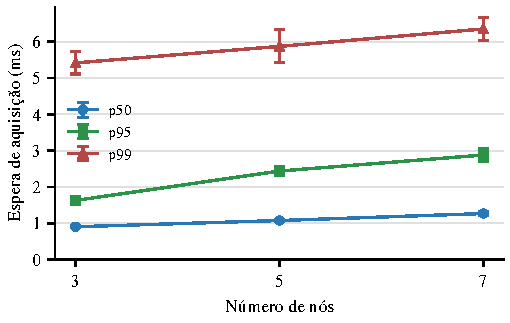
\includegraphics[width=\columnwidth]{figures/ra_latency.pdf}
\caption{Espera de aquisição RA. Cada ponto resume um percentil entre dez ensaios e as barras mostram IC95\%. A seção crítica de 5 ms não está incluída.}
\label{fig:ra}
\end{figure}

\subsection{Latência de aquisição e de registro}
A espera p95 de RA passou de 1,627~ms em três nós para 2,438~ms em cinco e 2,878~ms em sete. Cada novo participante recebe o pedido e precisa conceder permissão antes da entrada. A Figura~\ref{fig:ra} mostra o aumento também no p99. O experimento mede o efeito conjunto dessa comunicação, da disputa pela seção e do escalonamento dos processos.

\begin{figure}[!t]
\centering
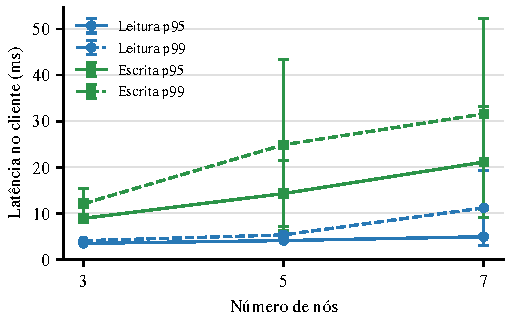
\includegraphics[width=\columnwidth]{figures/abd_latency.pdf}
\caption{Percentis p95 e p99 de latência ABD nas operações concluídas. Cor identifica leitura ou escrita e tracejado identifica p99. Barras indicam IC95\% entre ensaios.}
\label{fig:abd}
\end{figure}

No ABD, as médias do p99 de leitura foram 4,066, 5,349 e 11,209~ms para três, cinco e sete nós. Para escrita, foram 12,107, 24,898 e 31,585~ms. As escritas precisam persistir a nova versão antes da confirmação, mas o experimento não separa o custo de \texttt{fsync} dos demais custos. Os intervalos da Figura~\ref{fig:abd} ficam mais largos nas configurações maiores, principalmente no p99. Portanto, o aumento da média vem acompanhado de maior variação entre ensaios.

\subsection{Vazão e custo de comunicação}
A vazão ficou próxima da oferta configurada nos três tamanhos, como mostra a Figura~\ref{fig:vazao}. ABD concluiu em média 19,507, 19,650 e 19,678 operações/s, com oferta de 20/s. RA concluiu 9,712, 9,773 e 9,828, com oferta de 10/s. Por causa do sorteio Poisson, a oferta efetiva média foi de 9,913/s em RA e 20,007/s em ABD. As duas curvas representam cargas diferentes, não uma comparação de capacidade máxima.

\begin{figure}[!t]
\centering
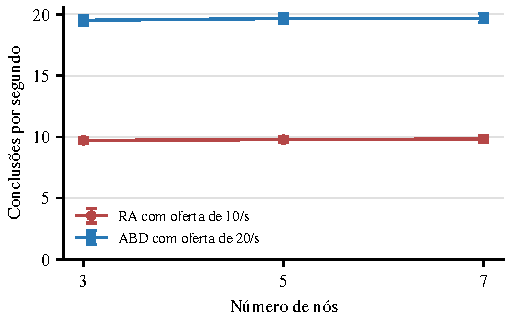
\includegraphics[width=\columnwidth]{figures/throughput.pdf}
\caption{Vazão concluída dentro da janela de medição, com média e IC95\%. As ofertas distintas estão indicadas na legenda e não representam saturação.}
\label{fig:vazao}
\end{figure}

A fração média de sucesso RA subiu de 97,99\% para 99,15\%. Uma explicação possível é a distribuição da mesma carga agregada entre mais coordenadores, reduzindo as recusas locais. Não variamos a carga até a saturação para verificar essa hipótese.

\begin{figure}[!t]
\centering
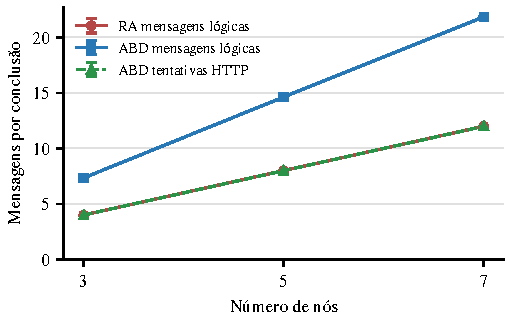
\includegraphics[width=\columnwidth]{figures/communication.pdf}
\caption{Comunicação por conclusão drenada, com média e IC95\%. Envelopes lógicos e tentativas HTTP são contagens diferentes. RA apresentou contagens coincidentes de envelopes e tentativas.}
\label{fig:mensagens}
\end{figure}

RA usou exatamente as $2(N-1)$ mensagens previstas, com 4, 8 e 12 por aquisição. Em ABD, contamos aproximadamente $2(N-1)$ tentativas HTTP por conclusão. A contagem de envelopes, que inclui respostas geradas, foi de 7,340, 14,629 e 21,850. Essa diferença aparece porque alguns envios são cancelados quando a maioria já respondeu. Esperar um quórum não significa enviar pedidos somente a esse quórum. Na Figura~\ref{fig:mensagens}, as contagens crescem linearmente com $N$.

\section{Falhas e retomada de progresso}
As Figuras~\ref{fig:particao} e~\ref{fig:crash} mostram a evolução temporal de conclusões e falhas. Cada segundo é agregado primeiro dentro de cada ensaio e depois entre as dez repetições. As bandas são IC95\%, com o eixo restrito a taxas não negativas. As regiões cinzas cobrem os comandos de injeção ou reconexão e a guarda posterior de 1~s. As linhas verticais indicam o término médio desses comandos. Os 40 ensaios somaram 20\,916 ofertas e 13\,149 conclusões drenadas.

\begin{figure*}[!t]
\centering
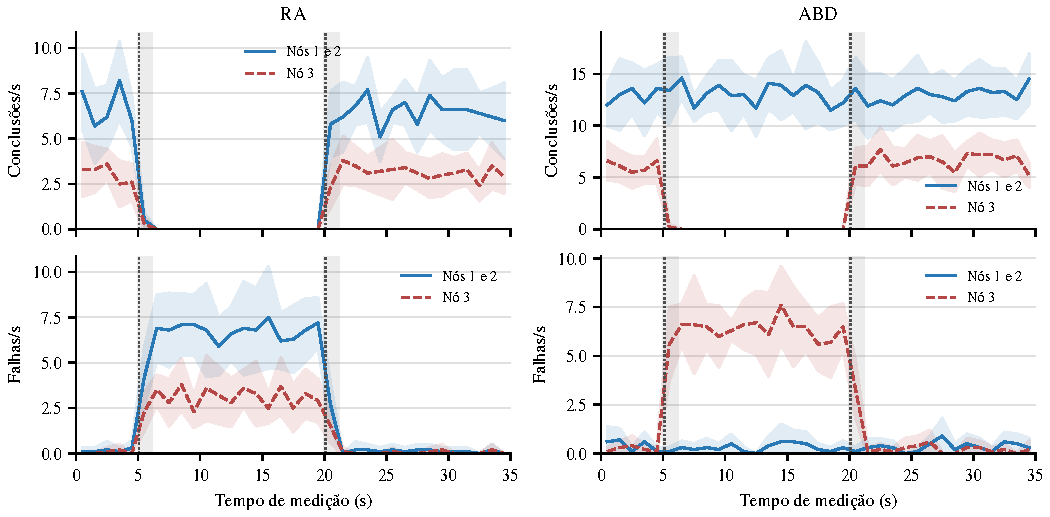
\includegraphics[width=\textwidth]{figures/partition.pdf}
\caption{Partição do nó 3 e posterior reconexão em três participantes. A linha superior mostra conclusões e a inferior mostra todos os desfechos malsucedidos. A maioria ABD continua concluindo operações, enquanto RA perde progresso nos dois lados. Após a reconexão, os dois protocolos voltam a concluir nos três nós. Bandas indicam IC95\% entre dez ensaios.}
\label{fig:particao}
\end{figure*}

\subsection{Partição e reconexão}
Durante o intervalo guardado de partição, RA não confirmou novas aquisições em nenhum lado. ABD manteve vazão de 13,152 conclusões/s na maioria, com IC95\% de 12,957 a 13,347. O nó isolado não concluiu operações. Houve invocações reais nesse nó e recusas HTTP~504, com identidade e saúde ainda acessíveis. Portanto, o bloqueio da minoria não foi inferido apenas de uma falha de conexão.

Depois da reconexão, novas invocações concluíram nos dois lados em todas as repetições. Até a primeira conclusão, medimos em média 0,309~s em RA, com IC95\% de 0,205 a 0,413, e 0,059~s em ABD, com IC95\% de 0,025 a 0,093. O gerador precisa emitir um novo pedido antes que ele possa terminar. Esses tempos incluem essa espera e foram medidos sob taxas diferentes, por isso não permitem afirmar que um protocolo se recupera mais rápido que o outro.

\begin{figure*}[!t]
\centering
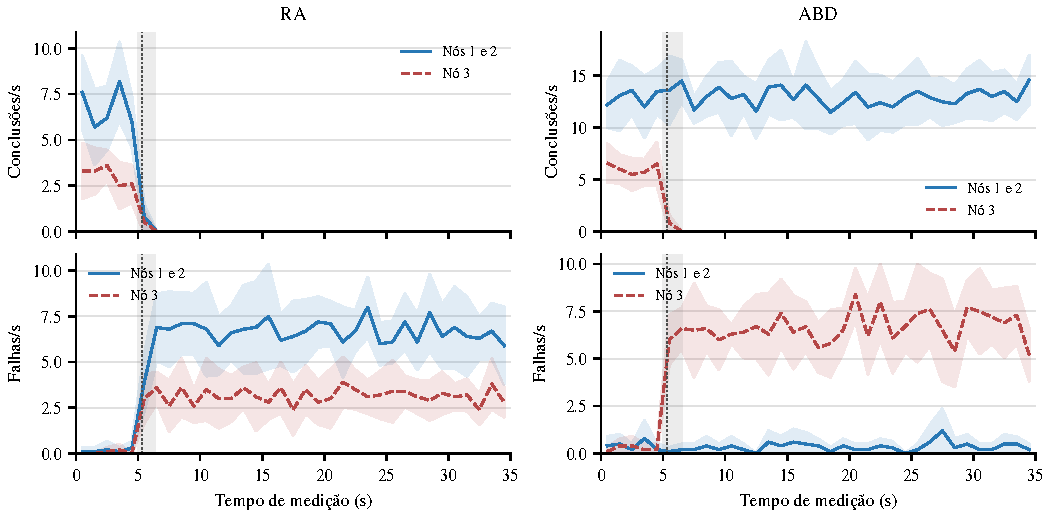
\includegraphics[width=\textwidth]{figures/crash.pdf}
\caption{Crash permanente do nó 3, sem reinício. RA deixa de concluir novas aquisições. ABD preserva operações nos nós 1 e 2. A série do nó morto mantém erros de transporte entre os desfechos malsucedidos, sem restringir falhas a timeouts. Bandas indicam IC95\% entre dez ensaios.}
\label{fig:crash}
\end{figure*}

\subsection{Crash permanente e erros}
Com o nó 3 morto, RA não concluiu novas aquisições. ABD manteve 12,996 conclusões/s nos outros dois nós, com IC95\% de 12,496 a 13,496. O contador integrado ficou bloqueado porque precisa adquirir RA antes de acessar o registro. A leitura ABD isolada continuou disponível.

Erros do processo morto podem ser imediatos, sem consumir o deadline. Por isso, os painéis inferiores incluem todos os desfechos malsucedidos. Escritas ABD sem resposta permanecem conservadoramente indeterminadas, sem afirmar aplicação ou rollback. Percentis calculados apenas sobre sucessos não descrevem essas tentativas. Como o nó morto não fornece snapshot final, não estimamos comunicação total do cluster nesse cenário.

\subsection{Correção do transporte no piloto}
No primeiro piloto, RA não voltou a concluir operações depois da reconexão, embora os endpoints estivessem acessíveis. O transporte HTTP ainda mantinha tentativas de conexão DNS e TCP após o cancelamento do pedido. Essas tentativas usavam o timeout padrão de 30~s e ocupavam os slots de conexão. Ajustamos o prazo de conexão para 500~ms nos dois protocolos e repetimos o cenário, com retomada dos três nós. Esse piloto foi preservado para diagnóstico, mas ficou fora dos resultados. Reiniciamos a coleta com a imagem corrigida antes dos cem ensaios.

\balance
\section{Limitações e conclusão}
Todos os contêineres executaram no mesmo computador e compartilharam CPU, disco, kernel e rede Docker. Uma falha de processo nesses testes não equivale à perda de uma máquina independente. Além disso, a memória disponível era limitada e a swap estava quase cheia, o que pode aumentar a variação das latências. As dez repetições medem essa variação no host usado, não a diferença entre computadores ou redes.

Variamos o número de nós. Também suportamos atraso e perda injetados no transporte, além de reintegração opcional, mas a campanha congelada de desempenho não os varre em todas as taxas. Não isolamos o custo da persistência. A associação é fixa e os pares são confiáveis. Os testes de correção cobrem execuções finitas e não substituem uma prova para todos os escalonamentos. Contêineres no mesmo host compartilham CPU, disco e rede.

Os comandos de reprodução estão no \href{../README.md}{README do T2}. A campanha preserva operações, eventos, logs, configuração e hashes. \texttt{frozen.json} registra taxas, sementes e ordem dos ensaios. As figuras usam \texttt{summary.json}. Históricos de correção estão em \texttt{data/abd/} e \texttt{data/integrated/}.

Rodrigo Camargo implementou o núcleo RA/ABD e a campanha. André Loubet estruturou o relatório e a análise. Gabriel Eiji M. M. Tomonari revisou o texto, o detector de falhas, a reintegração e o roteiro do vídeo. Atividades conjuntas: validação dos smokes e da entrega.

O principal resultado é a diferença de progresso. Sem um participante, RA não autoriza novas entradas; ABD ainda funciona com maioria. No contador, o incremento fica bloqueado por RA mesmo com o registro disponível. Aumentar o grupo elevou a comunicação e a espera de aquisição.


\begin{thebibliography}{9}
\bibitem{enunciado}
C.~A. Astudillo Trujillo e D.~M. da Cunha, ``Implementação de Algoritmos Distribuídos,'' enunciado do Trabalho~2, MC714, Instituto de Computação, Unicamp, out. 2026.
\bibitem{ricart}
G.~Ricart e A.~K. Agrawala, ``An optimal algorithm for mutual exclusion in computer networks,'' \emph{Communications of the ACM}, vol.~24, n.~1, pp.~9 a 17, 1981. \href{https://doi.org/10.1145/358527.358537}{10.1145/358527.358537}.
\bibitem{abd}
H.~Attiya, A.~Bar-Noy e D.~Dolev, ``Sharing memory robustly in message-passing systems,'' \emph{Journal of the ACM}, vol.~42, n.~1, pp.~124 a 142, 1995. \href{https://doi.org/10.1145/200836.200869}{10.1145/200836.200869}.
\bibitem{mwmr}
L.~Tseng, N.~Zhou, C.~Dumas, T.~Bantikyan e R.~Palmieri, ``Distributed multi-writer multi-reader atomic register with optimistically fast read and write,'' \emph{Proc. SPAA}, 2023. Seção~2.2 sobre ABD MWMR. \href{https://doi.org/10.1145/3558481.3591086}{10.1145/3558481.3591086}. Versão aberta em \href{https://arxiv.org/abs/2304.09382}{arXiv 2304.09382}.
\bibitem{linearizability}
M.~P. Herlihy e J.~M. Wing, ``Linearizability. A correctness condition for concurrent objects,'' \emph{ACM Transactions on Programming Languages and Systems}, vol.~12, n.~3, pp.~463 a 492, 1990. \href{https://doi.org/10.1145/78969.78972}{10.1145/78969.78972}.
\bibitem{t1}
R.~Camargo, A.~Loubet e G.~E.~M.~M.~Tomonari, ``Balanceador de Carga para um Sistema Distribuído,'' relatório do Trabalho~1, MC714, Unicamp, 2026.
\end{thebibliography}

\textit{Uso de IA:} utilizamos o ChatGPT para conferir trechos de código e derivações; decisões de projeto, implementação e resultados são dos autores.

\end{document}
